\documentclass[12pt,notitlepage,oneside]{report}

\usepackage{buetcseugthesis}

% Uncomment the following line if you need to write in Bangla
% \usepackage{usebangla}

% Uncomment any of the following lines should you need to
% suppress the LOF, or LOT or LOA

% \suppresslistoffigures 
% \suppresslistoftables
% \suppresslistofalgorithms

% For index creation, comment this out if you do not want to create an
% index
\makeindex[intoc]

\begin{document}

% Edit as needed below this line
% %%%%%%%%%%%%%%%%%%%%%%%%%%%%%%%%%%%%%%%%%%%%%%%%%%%%%%%%

% Chapter-1 Introduction
% \chapter{Introduction}\label{intro}

This chapter is for your introduction.

\section{Cross Referencing}
We have incorporated the \verb@\cref@ or \verb@\Cref@ command from
\texttt{cleveref} package in this system. This will automatically
insert words like Figure, Table etc.\ in your text.

See these examples:
\begin{itemize}
\item \Cref{fig:sample} is a sample figure.
\item \Cref{tab_our} is a table.
\item \Cref{sec:cite} in \Cref{ch:citations} shows some examples of
  citations.
\end{itemize}

\section{How to Write a Section}

This is for writing section.

\section{How to Add Table and Figures}\label{contribution}
You should refer a figure as, ``\Cref{fig:sample} is a sample
figure''.

\begin{figure}[!tb]
  \centering
  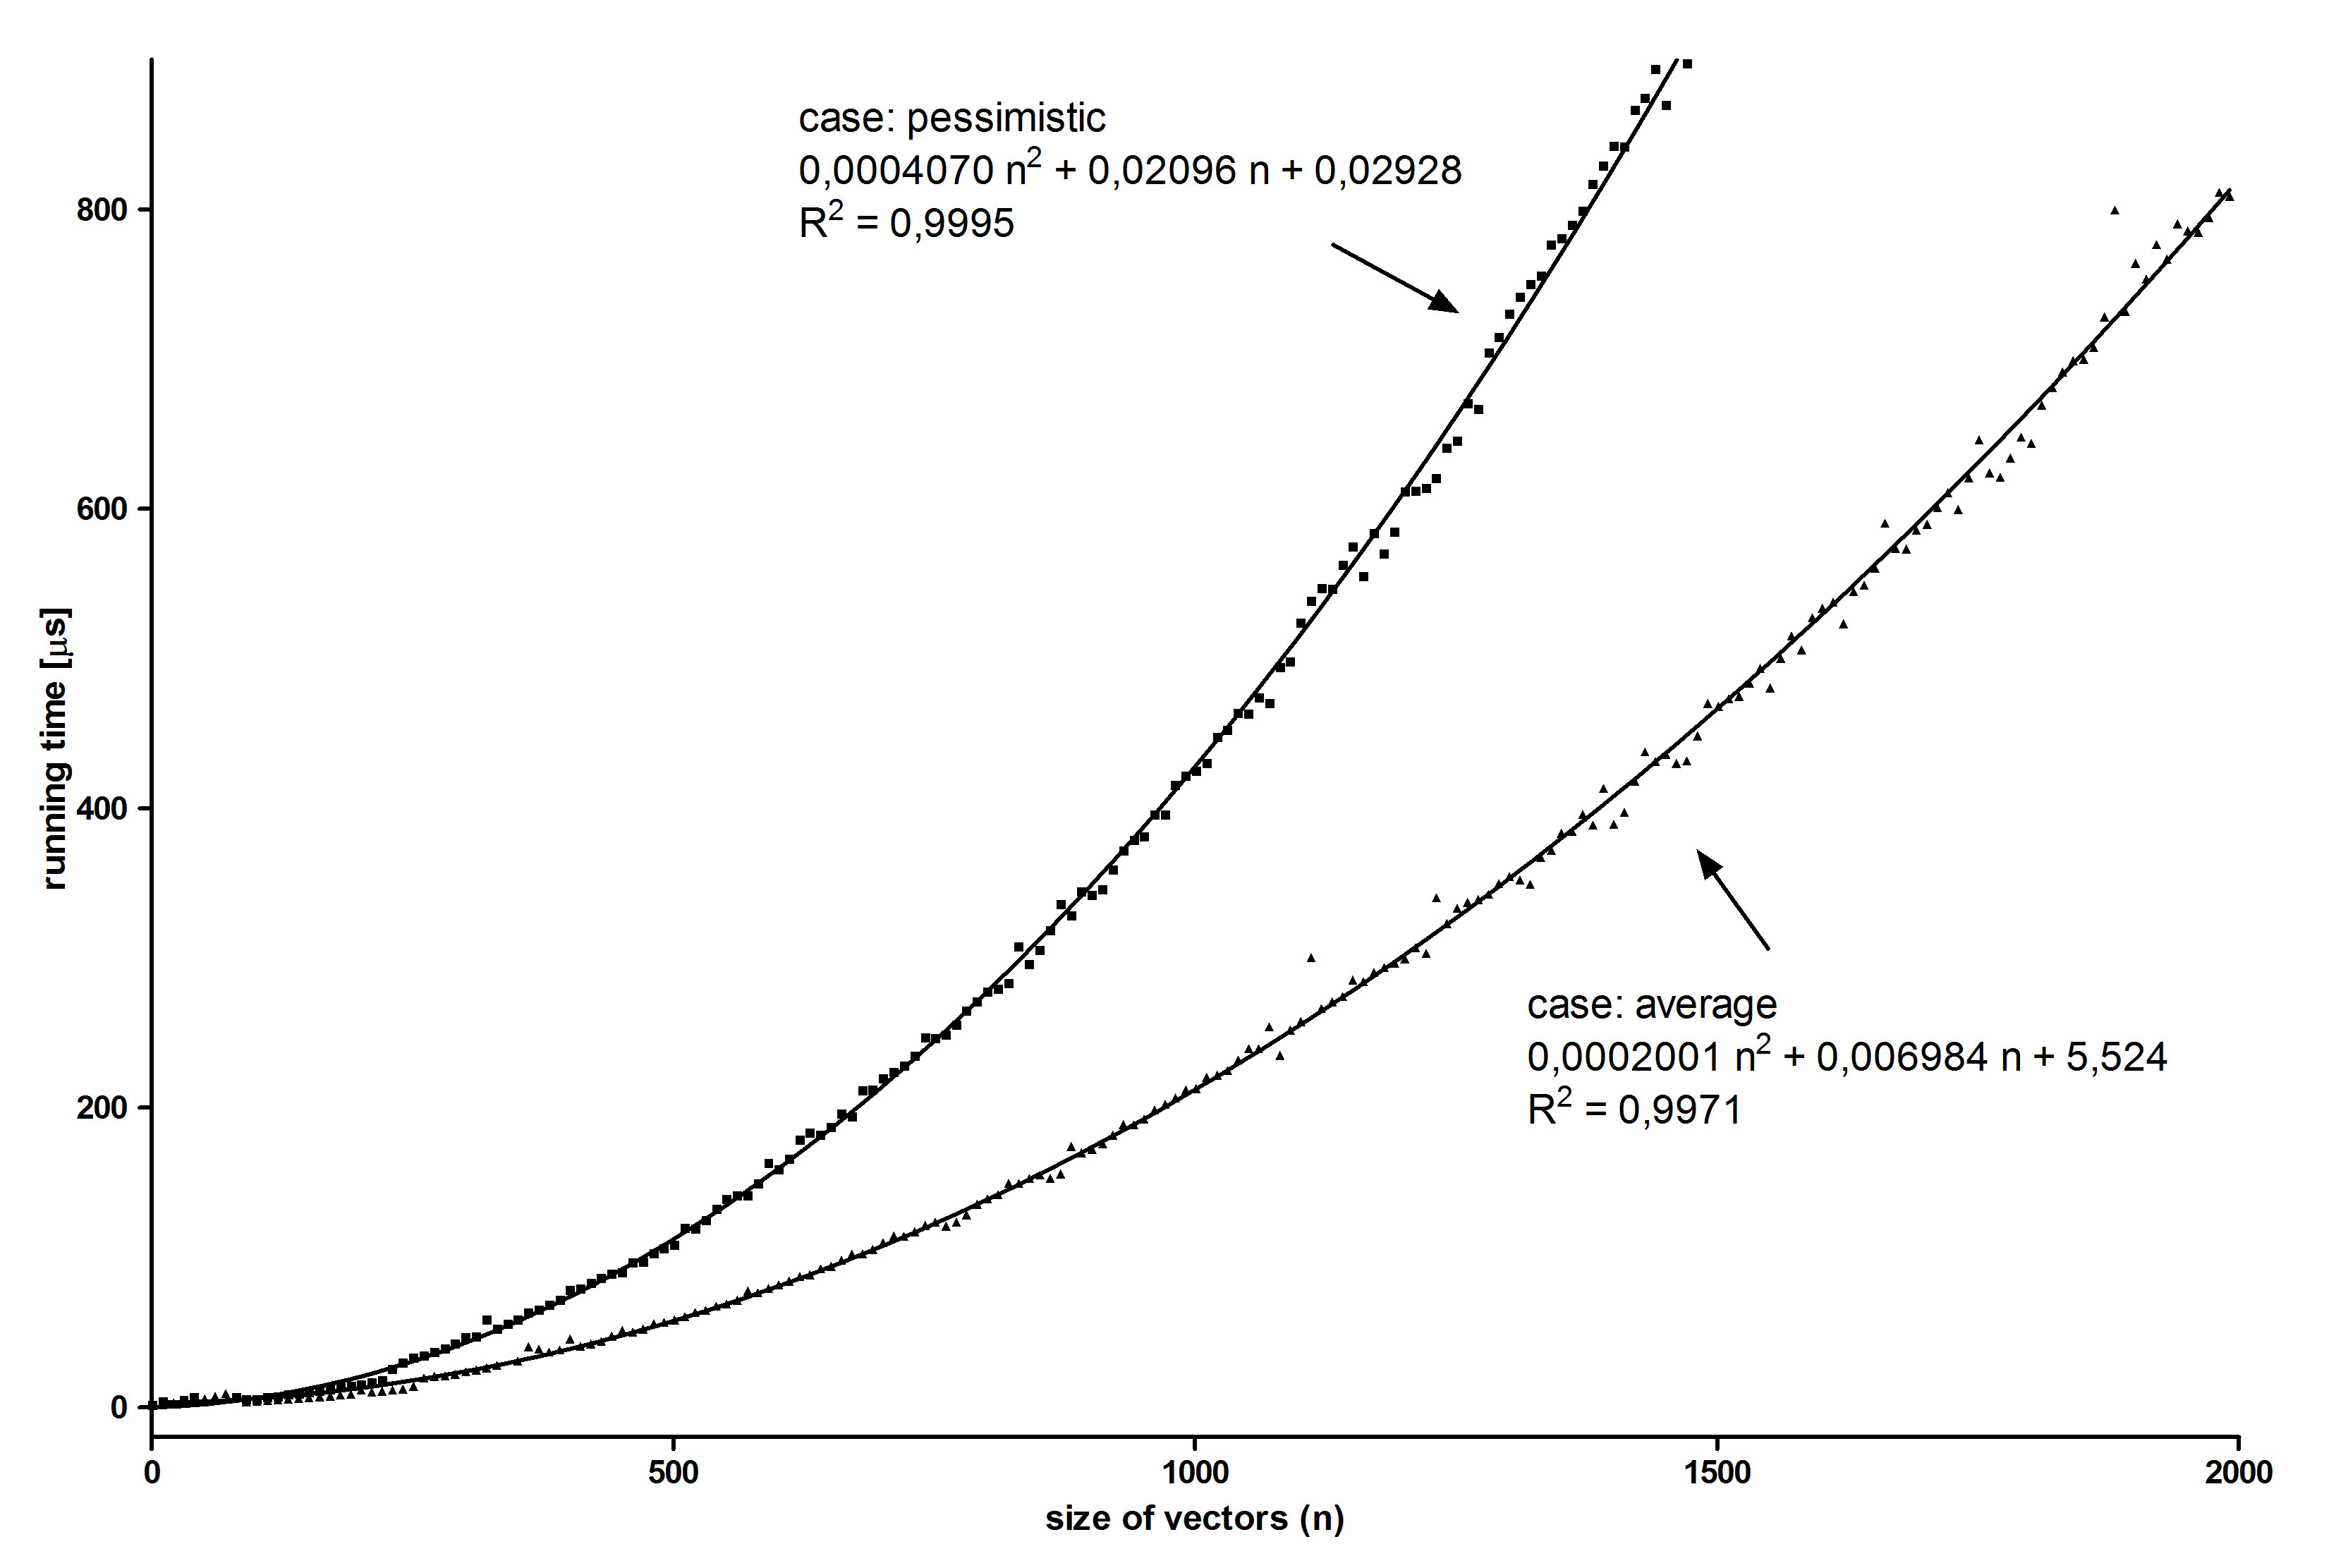
\includegraphics[width=0.9\textwidth]{figures/sample}
  \caption{This is a sample figure.}
  \label{fig:sample}
\end{figure}

				
Then we applied same test cases to our modified algorithm i.e.\ the
heuristic algorithm with our new operation \textit{Block Reversal}. The
performance is shown in \Cref{tab_our}.


\begin{table}[!tb]
  \begin{center}
    \caption{Performance table of \emph{Block reversal} in a heuristic algorithm}
    \label{tab_our}

    \begin{tabular}{|l|r|r|r|r|r|r|r|r|r|r|r|r|r|}
      \hline
      $\alpha$     & $\alpha n$ & \multicolumn{11}{c|}{Test Cases} & \multicolumn{1}{c|}{Average \# of}                                     \\
      \cline{3-13} &            & 1                                & 2  & 3  & 4  & 5  & 6  & 7  & 8  & 9  & 10 & 11 & calculated operation \\
      \hline
      0.1        & 2          & 2                                & 2	& 2  & 2  & 2  & 2  & 2  & 2  &	2  & 2	& 2  & 2                    \\
      0.2        & 4          & 4                                & 4	& 5  & 2  & 4  & 4  & 4  & 4  &	2  & 4	& 4  & 3.73                 \\
      0.3        & 6          & 5                                & 6	& 6  & 6  & 6  & 7  & 6  & 5  &	6  & 6	& 6  & 5.91                 \\
      0.4        & 8          & 7                                & 8	& 5  & 6  & 7  & 6  & 6  & 7  &	8  & 8	& 7  & 6.82                 \\
      0.5        & 10         & 9                                & 10	& 6  & 12 & 10 & 8  & 10 & 10 &	7  & 7	& 10 & 9                    \\
      0.6        & 12         & 9                                & 12	& 16 & 10 & 12 & 12 & 9  & 11 &	12 & 9	& 12 & 11.27                \\
      0.7        & 14         & 13                               & 7	& 18 & 15 & 14 & 8  & 13 & 11 &	13 & 13	& 14 & 12.64                \\
      0.8        & 16         & 10                               & 17	& 14 & 16 & 13 & 16 & 13 & 11 &	13 & 17	& 13 & 13.91                \\
      0.9        & 18         & 14                               & 16	& 15 & 12 & 15 & 11 & 15 & 11 &	15 & 12	& 12 & 13.45                \\
      1          & 20         & 18                               & 11	& 13 & 11 & 13 & 15 & 17 & 17 &	13 & 18	& 12 & 14.36                \\
      \hline
    \end{tabular}
  \end{center}
\end{table}


These are some dummy text used as page fillers only.

Lorem ipsum dolor sit amet, consectetur adipiscing elit. Cras et
ultricies massa. Nulla a sapien lobortis, dignissim nibh in, aliquet
mauris. Integer at dictum metus. Quisque in tortor congue ipsum
ultricies tristique. Maecenas ut tortor dapibus, sagittis enim at,
tincidunt massa. Ut sollicitudin sagittis ipsum, ac tincidunt quam
gravida ac. Nullam quis faucibus purus. Aliquam vel pretium
turpis. Aliquam a quam non ex interdum sagittis id vitae quam. Nullam
sodales ligula malesuada maximus consequat. Proin a justo eget lacus
vulputate maximus luctus vitae enim. Aliquam libero turpis, pharetra a
tincidunt ac, pulvinar sit amet urna. Pellentesque eget rutrum diam,
in faucibus sapien. Aenean sit amet est felis. Aliquam dolor eros,
porttitor quis volutpat eget, posuere a ligula. Proin id velit ac
lorem finibus pellentesque.

Maecenas vitae interdum mi. Aenean commodo nisl massa, at pharetra
libero cursus vitae. In hac habitasse platea dictumst. Suspendisse
iaculis euismod dui, et cursus diam. Nullam euismod, est ut dapibus
condimentum, lorem eros suscipit risus, sit amet hendrerit justo
tortor nec lorem. Morbi et mi eget erat bibendum porta. Ut tristique
ultricies commodo. Nullam iaculis ligula sed lacinia ornare.

Sed ultricies cursus nisi at vestibulum. Aenean laoreet viverra
efficitur. Ut eget sapien lorem. Mauris malesuada, augue in pulvinar
consectetur, ex tortor tristique ligula, sit amet faucibus metus
lectus interdum nisl. Nam eget turpis vitae ligula pulvinar bibendum a
ut ipsum. Mauris fringilla lacinia malesuada. Fusce id orci
velit. Donec tristique rhoncus urna, a hendrerit arcu vehicula
imperdiet. Integer tristique erat at gravida condimentum. Sed ornare
cursus quam, eget tincidunt enim bibendum sed. Aliquam elementum
ligula scelerisque leo sagittis, quis convallis elit dictum. Donec sit
amet orci aliquam, ultricies sapien nec, gravida nisi. Etiam et
pulvinar diam, et pellentesque arcu. Nulla interdum metus sed aliquet
consequat.

Proin in mi id nulla interdum aliquet ac quis arcu. Duis blandit
sapien commodo turpis hendrerit pharetra. Phasellus sit amet justo
orci. Proin mattis nisl dictum viverra fringilla. Interdum et
malesuada fames ac ante ipsum primis in faucibus. Curabitur facilisis
euismod augue vestibulum tincidunt. Nullam nulla quam, volutpat vitae
efficitur eget, porta sit amet nunc. Phasellus pharetra est eget urna
ornare volutpat. Aenean ultrices, libero eget porttitor fringilla,
purus tortor accumsan neque, sit amet viverra felis tortor eget
justo. Nunc id metus a purus tempus euismod condimentum non lacus. Nam
vitae diam aliquam, facilisis diam quis, pharetra nunc. Nulla eget
vestibulum tellus, ut cursus tellus. Vestibulum euismod pellentesque
sodales.

Maecenas at mi interdum, faucibus lorem sed, hendrerit nisi. In vitae
augue consequat diam commodo porta sit amet eu purus. Mauris mattis
condimentum feugiat. Nulla commodo molestie risus vitae maximus. Proin
hendrerit neque malesuada urna laoreet convallis. Etiam a diam
pulvinar, auctor sem ac, hendrerit risus. Ut urna urna, venenatis ac
tellus non, scelerisque tristique ligula. Vestibulum sollicitudin vel
leo malesuada accumsan. Donec sit amet erat diam. Vestibulum ante
ipsum primis in faucibus orci luctus et ultrices posuere cubilia
Curae; Vivamus odio dui, scelerisque et lorem egestas, posuere
ullamcorper nunc. Integer varius nunc nec velit tincidunt
commodo. Mauris rhoncus ultrices sapien non suscipit.


End of dummy text.


\endinput
\chapter{Introduction}\label{intro}
The present world is a place with immeasurable data or information due to World Wide Web.
 Where the web is a vast repository of knowledge. 
 Each and every day this amount is increasing .It is getting harder day by day 
 for a person to extract exact information s/he needs to analysis them to have a desired goal.



 But automatically extracting that huge knowledge at scale has proven to be a formidable challenge for computer science to organize, store and most importantly efficiently searching. A search data structure is any data structure that allows the efficient retrieval of specific items from a set of items, 
 such as a specific record from a database.


 A single word can represent a person, place, name of organization, restaurant. Again a word slightly different spelling can represent totally different thing. As far as the word efficient searching means searching a particular word with all its variations. It is very hard for a single person or a particular software to extracting the exact semantic data. It may be a better way for us to make machine learn the way of efficient searching.


 It may be helpful for us to write grammars for machine to learn than writing all the rules of searching by ourselves. Now for machine to learn to work or search in order to search efficiently we need data or information to be organized in a way that machine can analyze those data. Here knowledge graph comes into play.


 Knowledge graphs have become an increasingly crucial component in machine intelligence systems, powering ubiquitous digital assistants and inspiring several large scale academic projects across the globe. Many problems in AI require to deal with both relational structure and uncertainty. As a consequence, there is a growing need for tools that facilitate the development of complex probabilistic models with relational structure.



 All these facts are interrelated, and hence, recently this extracted knowledge has been referred to as a knowledge graph . A key challenge in producing the knowledge graph is incorporating noisy information from different sources in a consistent manner. Information extraction systems operate over many source documents, such as web pages, and use a collection of strategies to generate candidate facts from the documents, spanning syntactic, lexical and structural features of text. Ultimately, these extraction systems produce candidate facts that include a set of entities, attributes of these entities, and the relations between these entities which we refer to as the extraction graph.


 Recent evaluation efforts have focused on automatic knowledge base population [1,2], and many well-known broad domain and open information extraction systems exist, including the Never-Ending Language Learning (NELL) project [3], OpenIE [4], and efforts at Google [5], which use a variety of techniques to extract new knowledge, in the form of facts, from the web. 

With the goal of teaching machines to understand human conversations, one of the most fundamental components of a conversational understanding system is the semantic parser. Conversational semantic parsers map natural language (NL) to a formal representation of meaning, typically defined by the intent of the user and the associated arguments of the intent (slots or concepts) [1].


Considerable advancements in semantic parsing have been made possible by the availability of massive volumes of data from social media.
With the recent emergence of very large-scale semantic knowledge graphs (KGs) [7], it is now possible to add structure to the machine learning procedures developed above. Specifically, we have developed methods to enrich KGs with automatically annotated training data through unsupervised data mining methods. 


Our approach is large-scale multi-concept (entity, relation, fact) open domain semantic parsing. Our approach is web-scale, learning neural embedding for all the concepts of twitter. Also, while the other approaches rely on supervised training, our approach is unsupervised.  
We use microblogging and more particularly Twitter for the following reasons:
 Microblogging platforms are used by different people to express their opinion about different topics, thus it is a valuable source of people’s opinions.  Twitter contains an enormous number of text posts and it grows every day. The collected corpus can be arbitrarily large.  Twitter’s audience varies from regular users to celebrities, company representatives, politicians, and even country presidents. Therefore, it is possible to collect text posts of users from different social and interests groups.  Twitter’s audience is represented by users from many countries. 


 In this thesis paper we analyze the process, algorithm for constructing knowledge graph. We try to extract information from twitter. Moreover we develop the way of accessing DBpedia database in order to enrich entity relationship in knowledge graph. It means knowledge in graph form. Here nodes are entities which are labeled with attributes typed edges between two nodes capture a relationship between entities. KG is vastly used in google, Amazon as amazon product graph, Facebook graph API, IBM Watson, Microsoft satori.  Generally knowledge graph come from structured or unstructured texts and Images and videos. 


 In our KGs entity-relationship edge is assumed as RDF triples like <rdf: Subject, rdf: Predicate, rdf: Object >  .
A starting with GATE Developer 8.4.1 for analyzing live tweets from twitter many processing resources such as ANNIE, Transducer allowed us identifying Token of different kinds. By codding grammar rule using JAPE in GATE noun, pronoun were identified which will be used as Node in KGs. 


But for the seek of better semantic analysis and improved relationship between closer entity, development of a process ‘Word Hashing’ has been done. Which represents a word of a string as vector of a letter n-grams to reduce the dimensionality bag of words-term vectors. Two words are compared based on the angle between two vectors representing those words. The smaller the angle, the closer the relation between the words. 
So , our goal is to through all this process developing a better knowledge graph based on closer entity-relationship that is efficient to extract information , process and analyze .
\endinput

% Citation examples
% \chapter{Citation Examples}\label{ch:citations}

In this chapter we show how we can cite the references.


\section{See the Citations}
\label{sec:cite}

As discussed by authors
in~\cite{akbar2006solving,karim2015comograd,alam2012diversity} we can
further show how this affects
us. Moreover~\cite{kaykobad1987nonnegative,kaykobad1985positive,kaykobad19983,MCNC,guo2001floorplanning,holland1975as,aickelin2005artificial,al2010artificial}
can be examples for the previous works. Among
these~\cite{aickelin2005artificial,faruque2016modelling,durocher2015graphs,rahman2016absent,hashem2013countering,farhad2016mapping,malek2016balanced}
are the prominent ones. Also you can take a look
at~\cite{bashir2016learning,uddin2014citizen,kamal2016boosting,haque2013constructing,mukta2016identifying,ali2016spatial,islam2009new,al2010stable}.


\endinput




\chapter{Related Works}\label{intro}
Previously there have been many researches conducted on knowledge graphs.
Most of them primarily identify major terms or keywords, remove noise, 
fetching missing information and disambiguate them to appropriate topic.
 

 
To disambiguate and relate a concept with similar concept,
researchers have used Probabilistic Soft Logic (PSL) withontological constraints,  
identify coreferences etc, as well as machine learning, deep neural networks.
There are many links among different concepts. Mihalcea annd Csomai et al worked onlink detection. 
Their work is on linking phrases to appropriate concept. To disambiguate in link detetion, they 
took help of the surrounding words ( the words themselves and their parts of speech), and compare with training data.
After that, in order to organize the documents, they have used topic indexing.
In order to make link detection efficient, Mihalcea annd Csomai et al used (a) commonness (prior probability 
of each sense) and (b) how the sense relate with the nearby context.


 
Next we have an important work of Larry Heck and Hongzhao Huang. First they developed a robust way to represent concepts.
 Many NLP tools use string concatenation to represent ideas.
But most of the time it fails to represent appropriate concepts. For example 'Madrid' is a place, 'Real' means 
something authentic or true, but 'Real Madrid' referres to a football club. This is a counter example where string concatenation fails.
A possible alternative is to use word hashing with n-gram (tri-gram) word representation. This way can be
 used to represent any words that are not even seen before. After that they did neural embedding of knowledge graph. 
 To do so, they tracked a concept and its corresponding subgraph, encode the knowledge as featured vector.
 then they trained Deep Neural Network to get semantic relationship.

 





\endinput
\chapter{Tentative Methodology}\label{ch3}
In order to create a graph $G = <V,E>$, where set of vertices is $V = <v_1,v_2,... v_n>$ and
set of edges $E = <e_1, e_2,...,e_m>$. Here vertex $v_i = <m_i, c_i>$ where $m_i$ is a tweet and $c_i$
is a concept from dbpedia.
So each node is a pair of tweeter mention $m_i$ and its corresponding concept $c_i$.

To create the nodes, we need to collect tweets. But the tweets donot give adequate data. 
Since a single tweet doesnot give us adequate data, we can use a set of tweets discuss about same topic 
leading us to some data to disambiguate meaning. In order to work with tweets, we need to 
perform some Natural Language Processing. For this we will use GATE Developer ~\cite{url0gate} , a 
text analysis or language processing toolkit. It helps us to annotate, gazetize, corefer
 etc in the tweets.


Next we need to collect data from dbpedia because the tweets themselves 
donot provide adequate data. After collecting the dbpedia data, we will convert them into $n$-grams.
For each acticles in dbpedia, we will create its corresponding concept vector, $c$. After that, we need to 
use machine learning to train how to detect a concept and find relations between them. We also need 
to train on matching twitter mentions $m$ with their corresponding concept vectors $c$.
 
 Thus we will have nodes $<m_i, c_i>$. After that, we need to connect the nodes with edges. 
 We will use link detection tecniques as discussed in ~\cite{ref3LinkWikipedia} to 
 find possible links and disambiguate links.


\endinput
% Another chapter
%\chapter{Another Chapter}\label{anotherchapter}


\section{A Section}
Some text.
\subsection{This is a Subsection}
And some more.
\subsubsection{This is a Subsubsection}
Yet some more.

\section{And Another Section}

Here are some dummy texts.

Lorem ipsum dolor sit amet, consectetur adipiscing elit. Cras et
ultricies massa. Nulla a sapien lobortis, dignissim nibh in, aliquet
mauris. Integer at dictum metus. Quisque in tortor congue ipsum
ultricies tristique. Maecenas ut tortor dapibus, sagittis enim at,
tincidunt massa. Ut sollicitudin sagittis ipsum, ac tincidunt quam
gravida ac. Nullam quis faucibus purus. Aliquam vel pretium
turpis. Aliquam a quam non ex interdum sagittis id vitae quam. Nullam
sodales ligula malesuada maximus consequat. Proin a justo eget lacus
vulputate maximus luctus vitae enim. Aliquam libero turpis, pharetra a
tincidunt ac, pulvinar sit amet urna. Pellentesque eget rutrum diam,
in faucibus sapien. Aenean sit amet est felis. Aliquam dolor eros,
porttitor quis volutpat eget, posuere a ligula. Proin id velit ac
lorem finibus pellentesque.

Maecenas vitae interdum mi. Aenean commodo nisl massa, at pharetra
libero cursus vitae. In hac habitasse platea dictumst. Suspendisse
iaculis euismod dui, et cursus diam. Nullam euismod, est ut dapibus
condimentum, lorem eros suscipit risus, sit amet hendrerit justo
tortor nec lorem. Morbi et mi eget erat bibendum porta. Ut tristique
ultricies commodo. Nullam iaculis ligula sed lacinia ornare.

Sed ultricies cursus nisi at vestibulum. Aenean laoreet viverra
efficitur. Ut eget sapien lorem. Mauris malesuada, augue in pulvinar
consectetur, ex tortor tristique ligula, sit amet faucibus metus
lectus interdum nisl. Nam eget turpis vitae ligula pulvinar bibendum a
ut ipsum. Mauris fringilla lacinia malesuada. Fusce id orci
velit. Donec tristique rhoncus urna, a hendrerit arcu vehicula
imperdiet. Integer tristique erat at gravida condimentum. Sed ornare
cursus quam, eget tincidunt enim bibendum sed. Aliquam elementum
ligula scelerisque leo sagittis, quis convallis elit dictum. Donec sit
amet orci aliquam, ultricies sapien nec, gravida nisi. Etiam et
pulvinar diam, et pellentesque arcu. Nulla interdum metus sed aliquet
consequat.

Proin in mi id nulla interdum aliquet ac quis arcu. Duis blandit
sapien commodo turpis hendrerit pharetra. Phasellus sit amet justo
orci. Proin mattis nisl dictum viverra fringilla. Interdum et
malesuada fames ac ante ipsum primis in faucibus. Curabitur facilisis
euismod augue vestibulum tincidunt. Nullam nulla quam, volutpat vitae
efficitur eget, porta sit amet nunc. Phasellus pharetra est eget urna
ornare volutpat. Aenean ultrices, libero eget porttitor fringilla,
purus tortor accumsan neque, sit amet viverra felis tortor eget
justo. Nunc id metus a purus tempus euismod condimentum non lacus. Nam
vitae diam aliquam, facilisis diam quis, pharetra nunc. Nulla eget
vestibulum tellus, ut cursus tellus. Vestibulum euismod pellentesque
sodales.

Maecenas at mi interdum, faucibus lorem sed, hendrerit nisi. In vitae
augue consequat diam commodo porta sit amet eu purus. Mauris mattis
condimentum feugiat. Nulla commodo molestie risus vitae maximus. Proin
hendrerit neque malesuada urna laoreet convallis. Etiam a diam
pulvinar, auctor sem ac, hendrerit risus. Ut urna urna, venenatis ac
tellus non, scelerisque tristique ligula. Vestibulum sollicitudin vel
leo malesuada accumsan. Donec sit amet erat diam. Vestibulum ante
ipsum primis in faucibus orci luctus et ultrices posuere cubilia
Curae; Vivamus odio dui, scelerisque et lorem egestas, posuere
ullamcorper nunc. Integer varius nunc nec velit tincidunt
commodo. Mauris rhoncus ultrices sapien non suscipit.


Lorem ipsum dolor sit amet, consectetur adipiscing elit. Cras et
ultricies massa. Nulla a sapien lobortis, dignissim nibh in, aliquet
mauris. Integer at dictum metus. Quisque in tortor congue ipsum
ultricies tristique. Maecenas ut tortor dapibus, sagittis enim at,
tincidunt massa. Ut sollicitudin sagittis ipsum, ac tincidunt quam
gravida ac. Nullam quis faucibus purus. Aliquam vel pretium
turpis. Aliquam a quam non ex interdum sagittis id vitae quam. Nullam
sodales ligula malesuada maximus consequat. Proin a justo eget lacus
vulputate maximus luctus vitae enim. Aliquam libero turpis, pharetra a
tincidunt ac, pulvinar sit amet urna. Pellentesque eget rutrum diam,
in faucibus sapien. Aenean sit amet est felis. Aliquam dolor eros,
porttitor quis volutpat eget, posuere a ligula. Proin id velit ac
lorem finibus pellentesque.

Maecenas vitae interdum mi. Aenean commodo nisl massa, at pharetra
libero cursus vitae. In hac habitasse platea dictumst. Suspendisse
iaculis euismod dui, et cursus diam. Nullam euismod, est ut dapibus
condimentum, lorem eros suscipit risus, sit amet hendrerit justo
tortor nec lorem. Morbi et mi eget erat bibendum porta. Ut tristique
ultricies commodo. Nullam iaculis ligula sed lacinia ornare.

Sed ultricies cursus nisi at vestibulum. Aenean laoreet viverra
efficitur. Ut eget sapien lorem. Mauris malesuada, augue in pulvinar
consectetur, ex tortor tristique ligula, sit amet faucibus metus
lectus interdum nisl. Nam eget turpis vitae ligula pulvinar bibendum a
ut ipsum. Mauris fringilla lacinia malesuada. Fusce id orci
velit. Donec tristique rhoncus urna, a hendrerit arcu vehicula
imperdiet. Integer tristique erat at gravida condimentum. Sed ornare
cursus quam, eget tincidunt enim bibendum sed. Aliquam elementum
ligula scelerisque leo sagittis, quis convallis elit dictum. Donec sit
amet orci aliquam, ultricies sapien nec, gravida nisi. Etiam et
pulvinar diam, et pellentesque arcu. Nulla interdum metus sed aliquet
consequat.

Proin in mi id nulla interdum aliquet ac quis arcu. Duis blandit
sapien commodo turpis hendrerit pharetra. Phasellus sit amet justo
orci. Proin mattis nisl dictum viverra fringilla. Interdum et
malesuada fames ac ante ipsum primis in faucibus. Curabitur facilisis
euismod augue vestibulum tincidunt. Nullam nulla quam, volutpat vitae
efficitur eget, porta sit amet nunc. Phasellus pharetra est eget urna
ornare volutpat. Aenean ultrices, libero eget porttitor fringilla,
purus tortor accumsan neque, sit amet viverra felis tortor eget
justo. Nunc id metus a purus tempus euismod condimentum non lacus. Nam
vitae diam aliquam, facilisis diam quis, pharetra nunc. Nulla eget
vestibulum tellus, ut cursus tellus. Vestibulum euismod pellentesque
sodales.

Maecenas at mi interdum, faucibus lorem sed, hendrerit nisi. In vitae
augue consequat diam commodo porta sit amet eu purus. Mauris mattis
condimentum feugiat. Nulla commodo molestie risus vitae maximus. Proin
hendrerit neque malesuada urna laoreet convallis. Etiam a diam
pulvinar, auctor sem ac, hendrerit risus. Ut urna urna, venenatis ac
tellus non, scelerisque tristique ligula. Vestibulum sollicitudin vel
leo malesuada accumsan. Donec sit amet erat diam. Vestibulum ante
ipsum primis in faucibus orci luctus et ultrices posuere cubilia
Curae; Vivamus odio dui, scelerisque et lorem egestas, posuere
ullamcorper nunc. Integer varius nunc nec velit tincidunt
commodo. Mauris rhoncus ultrices sapien non suscipit.


\endinput

% Chapter showing example of index creation
%\chapter{Index Creation}
\section{BUET}
Bangladesh University of Engineering and Technology, abbreviated as
BUET\index{BUET}, is one of the most prestigious institutions for
higher studies in the country. About 5500 students are pursuing
undergraduate\index{BUET!undergraduate} and
postgraduate\index{BUET!postgraduate} studies in engineering,
architecture, planning and science in this institution. At present,
BUET has sixteen teaching departments under five faculties and it has
three institutes. Every year the intake of undergraduate students is
around 900, while the intake of graduate students in Master's and PhD
programs is around 1000. A total of about five hundred teachers are
teaching in these departments and institutes. There are additional
teaching posts like Dr.\ Rashid Professor, Professor Emeritus and
Supernumerary Professors.
 
\section{Campus}
The BUET campus is in the heart of Dhaka\index{Dhaka} --- the capital
city of Bangladesh. It has a compact campus with halls of residence
within walking distances of the academic buildings. The physical
expansion of the University over the last three decades has been
impressive with construction of new academic buildings,
auditorium\index{BUET!auditorium} complex, halls of residence, etc.
 
\section{History}\index{BUET!History}
BUET is the oldest institution for the study of Engineering and
Architecture in Bangladesh. The history of this institution dates back
to the days of Dhaka Survey School which was established at
Nalgola\index{Nalgola}, in Old Dhaka in 1876 to train Surveyors for
the then Government of Bengal of British India. As the years passed,
the Survey School became the Ahsanullah School of
Engineering\index{Ahsanullah School of Engineering} offering
three-year diploma courses in Civil, Electrical and Mechanical
Engineering. In recognition of the generous financial contribution
from the then Nawab of Dhaka, it was named after his father Khawja
Ahsanullah. It moved to its present premises in 1912. In 1947, the
School was upgraded to Ahsanullah Engineering College as a Faculty of
Engineering under the University of Dhaka, offering four-year
bachelor’s courses in Civil, Electrical, Mechanical, Chemical and
Metallurgical Engineering. In order to create facilities for
postgraduate studies and research, Ahsanullah Engineering College was
upgraded to the status of a University in 1962 and was named East
Pakistan University of Engineering and Technology. After the War of
Liberation in 1971\index{1971|see {War of Liberation}}\index{War of
  Liberation}, Bangladesh became an independent state and the
university was renamed as the Bangladesh University of Engineering and
Technology.
 
\section{Students}
Till today, it has produced around 25,000 graduates in different
branches of engineering and architecture, and has established a good
reputation all over the world for the quality of its graduates, many
of whom have excelled in their profession in different parts of the
globe. It was able to attract students from countries like
India\index{India}, Nepal\index{Nepal}, Iran\index{Iran},
Jordan\index{Jordan}, Malaysia\index{Malaysia}, Sri Lanka\index{Sri
  Lanka}, Pakistan\index{Pakistan} and Palestine\index{Palestine}.
 
\section{Departments}
Both Undergraduate and Postgraduate studies and research are now among
the primary functions of the University. Eleven departments under five
faculties offer Bachelor Degrees, while most of the departments and
institutes offer Master's Degrees and some of the departments have
Ph.D. programs. In addition to its own research programs, the
university undertakes research programs sponsored by outside
organizations like European Union, UNO,
Commonwealth\index{Commonwealth}, UGC\index{UGC}, etc. The expertise
of the University teachers and the laboratory facilities of the
University are also utilized to solve problems and to provide
up-to-date engineering and technological knowledge to the various
organizations of the country.


\endinput 

% Bangla example, uncomment if you need this
% \chapter{Example of Bangla}

\section{Long Text in English}

This text is in English.

\bengalitext{আর এটা বাংলায় লেখা।}

Lorem ipsum dolor sit amet, consectetur adipiscing elit. Cras et
ultricies massa. Nulla a sapien lobortis, dignissim nibh in, aliquet
mauris. Integer at dictum metus. Quisque in tortor congue ipsum
ultricies tristique. Maecenas ut tortor dapibus, sagittis enim at,
tincidunt massa. Ut sollicitudin sagittis ipsum, ac tincidunt quam
gravida ac. Nullam quis faucibus purus. Aliquam vel pretium
turpis. Aliquam a quam non ex interdum sagittis id vitae quam. Nullam
sodales ligula malesuada maximus consequat. Proin a justo eget lacus
vulputate maximus luctus vitae enim. Aliquam libero turpis, pharetra a
tincidunt ac, pulvinar sit amet urna. Pellentesque eget rutrum diam,
in faucibus sapien. Aenean sit amet est felis. Aliquam dolor eros,
porttitor quis volutpat eget, posuere a ligula. Proin id velit ac
lorem finibus pellentesque.

\section{Long Text in Bangla}

\begin{bengali}
  মধ্যাহ্ন বিরতির পর রানের চাকা বেশ দ্রুতই ঘোরাচ্ছিলেন মুরালি বিজয় আর
  চেতেশ্বর পূজারা। ১৭৮ রানের জুটি গড়েছিলেন তাঁরা। অবশেষে মেহেদী হাসান
  মিরাজের বলে স্বস্তি ফিরেছে বাংলাদেশ-শিবিরে। তাঁর বলে মুশফিকুর রহিমকে ক্যাচ
  দিয়েছেন চেতেশ্বর পূজারা। আউট হওয়ার আগে করেছেন ৮৩ রান। অপর প্রান্তে মুরালি
  বিজয় অপরাজিত ৯৩ রানে। এ প্রতিবেদন লেখার সময় ভারতের সংগ্রহ ২ উইকেটে
  ২০১। উইকেটে এসেছেন বিরাট কোহলি।

  বিজয়-পূজারা জুটি বেশ আগেই শেষ করে দেওয়ার সুযোগ এসেছিল বাংলাদেশের সামনে।
  বিজয়কে রান আউট করার সুযোগ পেয়েও তা কাজে লাগাতে পারেননি মিরাজ।

  তাঁর করা ১৯তম ওভারের তৃতীয় বলটি স্কয়ার লেগের দিকে ঘুরিয়েছিলেন মুরালি
  বিজয়। স্কয়ার লেগে ডাইভ দিয়ে রান বাঁচান কামরুল ইসলাম। কিন্তু নন স্ট্রাইকিং
  প্রান্তের চেতেশ্বর পূজারা রানটি পুরো করার জন্য দৌড়ালে প্রথমে বিজয় সাড়া দিতে
  চাননি। দুই ব্যাটসম্যানই ছিলেন একই প্রান্তে। পরে বিজয় নন স্ট্রাইকিং প্রান্তের
  দিকে দৌড় শুরু করেন। কামরুলের থ্রো বোলার মিরাজ ঠিকমতো ধরতে না পারায়
  নিশ্চিত রান আউটের হাত থেকে বেঁচে যান বিজয়।
\end{bengali}

% Chapter with math in ttile
%\chapter{$k$-safe Labeling of Petersen Graph}\label{safeklabelingpetersen}

In 1898, Petersen produced a trivalent graph with no leaves, now
called the Petersen graph~\cite{holton1993petersen}.  In this chapter
we study $k$-safe labeling for the Petersen graph. We also give upper
bound for the span of the Petersen graph. We provide necessary proof
for the upper bound.

\endinput



% Bibliographies and appendices
% You do not need to change anything in this file. If you want to
% change the reference style, comment/uncomment the \bibliographystyle
% lines

\clearpage
\renewcommand\bibname{References}
\addcontentsline{toc}{chapter}{References}

% Comment/uncomment as suits you
\bibliographystyle{ieeetr} %% IEEE transaction style
% \bibliographystyle{acm} %% ACM style
% \bibliographystyle{alpha}
\bibliography{buetcseugthesis}

\endinput


% Index, comment this out if you do not want to create an index
\printindex

\appendix
% Algorithms
\chapter{Algorithms}\label{ch:algorithms}

\section{Sample Algorithm}
In Algorithm~\ref{alg1} we show how to calcute $y=x^n$.

\begin{algorithm}
  \caption{Calculate $y = x^n$}
  \label{alg1}
  \begin{algorithmic}
    \input{algorithms/yxn.alg}
  \end{algorithmic}
\end{algorithm}

\endinput


% Codes
% Code settings
\lstset{
  language=C, % C, C++, Java, SQL are from the around hundred available
  basicstyle=\ttfamily,
  numbers=left,
  numberstyle=\footnotesize,
  stepnumber=1, 
  numbersep=2.0mm}

\chapter{Codes}\label{ch:codes}

\section{Sample Code}

We use this code to find out\dots

\lstinputlisting{codes/fibonacci.c}


\section{Another Sample Code}

\lstinputlisting[language=SQL,basicstyle=\small\ttfamily]{codes/salesa1.sql}

\endinput


\end{document}
